\documentclass[12pt]{article}
\usepackage{iftex}
\ifPDFTeX
  \PackageError{Treasury_PCA_Butterfly_Relative_Value}{Compile with LuaLaTeX or XeLaTeX}{Run `lualatex Treasury_PCA_Butterfly_Relative_Value.tex`.}
\fi
\usepackage{fontspec}
\defaultfontfeatures{Ligatures=TeX}
\IfFontExistsTF{Times New Roman}{\setmainfont{Times New Roman}}{\setmainfont{TeX Gyre Termes}}
\usepackage[a4paper,top=0.85in,bottom=0.85in,left=0.95in,right=0.95in]{geometry}
\usepackage{amsmath,amssymb,booktabs,graphicx,float,array,tabularx,hyperref,setspace,titlesec}
\hypersetup{colorlinks=true,linkcolor=black,urlcolor=blue,citecolor=black}
\setstretch{1.05}
\titlespacing*{\section}{0pt}{12pt plus 2pt minus 1pt}{6pt plus 1pt}
\titlespacing*{\subsection}{0pt}{8pt plus 2pt minus 1pt}{4pt plus 1pt}
\setlength{\floatsep}{8pt}
\setlength{\textfloatsep}{10pt}
\setlength{\intextsep}{8pt}
\setlength{\abovecaptionskip}{4pt}
\setlength{\belowcaptionskip}{2pt}
\newcolumntype{L}[1]{>{\raggedright\arraybackslash}p{#1}}
\sloppy

\title{\vspace{-0.5cm}Treasury PCA Butterflies, Carry, and Relative-Value Discipline}
\author{Dhruv Kohli}
\date{}

\begin{document}
\maketitle
\vspace{-0.5cm}
\noindent\rule{\textwidth}{0.4pt}

\begin{abstract}
This paper answers whether a PCA-neutral 2s5s10s Treasury butterfly isolates a tradable
curvature residual or only creates a clean-looking factor signal. We estimate Treasury
principal components on daily yield changes, construct exact and regularized butterflies, test
stationarity and walk-forward hedge stability, and then add carry/rolldown, transaction costs,
volatility targeting, purged validation, and actual-bond implementation diagnostics. The evidence is
deliberately conservative. The exact full-sample butterfly is neutral to level and slope by
construction, but the spread is not strongly stationary, rolling exact hedge ratios become unstable,
and stricter mean-reversion variants lose money after realistic filters. The carry-aligned momentum
branch is the least-rejected research branch, not a strong strategy result. Its 0.18 annualized
Sharpe is too weak for deployment, but useful because it shows which economic direction survives
after the naive PCA residual trade fails. That branch earns 307.47 bp in the fixed-maturity research
proxy, while CPCV, nested blocked selection, block bootstraps, empirical EGARCH full-curve nulls,
and bond-mapping diagnostics keep the claim modest. The trading conclusion is narrower: factor
neutrality is not alpha, and promotion to live capital requires executable instruments, financing,
costs, and risk controls.
\end{abstract}

\noindent\rule{\textwidth}{0.4pt}

\section{Introduction}

Treasury relative-value trades often start with a simple desk intuition: broad yield-curve moves can
be decomposed into level, slope, and curvature, and a butterfly can isolate what remains. In the
2s5s10s version, the trade owns the wings against the 5Y belly. The construction looks attractive
because it appears to remove the obvious macro duration bet while retaining exposure to curve
shape.

The problem is that factor neutrality is not the same as edge. A portfolio can have zero exposure to
the first two principal components and still fail for reasons that matter in actual rates trading:
the residual may not mean-revert, estimated loadings may be sample-dependent, exact hedge ratios
may create hidden gross exposure, carry may work against the signal, and the clean fixed-maturity
curve may not map cleanly into securities. This paper is built around those failure modes.

The analysis therefore moves in stages. First, it reconstructs the classical PCA butterfly carefully:
PCA is run on yield changes rather than yield levels, covariance PCA is used for hedge construction,
and exact 2s5s10s weights are solved to neutralize level and slope. Second, it asks whether that
residual has usable trading properties. Third, after the naive mean-reversion story weakens, it
rebuilds the trade with regularized hedge weights,
carry/rolldown, costs, volatility targeting, purged validation, full-curve null simulations, and
actual-bond mapping checks.

The so what is direct. A PCA-neutral Treasury butterfly is not alpha by itself. The contribution of
this project is showing how a clean curve residual survives or fails once the work imposes carry,
hedge instability, turnover, costs, validation discipline, and instrument mapping. In this sample,
the naive residual-fading story fails. Regularized hedge construction is cleaner, and carry-aligned
curvature momentum is the only branch left worth more execution research. The useful output is not
the 0.18 Sharpe. It is the ability to reject the first attractive chart and preserve only the part of
the idea that still makes economic sense.

\section{Related Literature and Research Design}\label{sec:literature}

The factor setup follows Litterman and Scheinkman \cite{littermanscheinkman1991}, who show that
level, slope, and curvature explain most Treasury yield-curve variation. This paper uses that
result as a construction tool rather than a trading conclusion. The return-predictability motivation
is related to Cochrane and Piazzesi \cite{cochranepiazzesi2005}, while the implementation caution
is closer to fixed-income arbitrage work such as Duarte, Longstaff, and Yu
\cite{duartelongstaffyu2007}, where apparent relative value must be interpreted through leverage,
drawdowns, liquidity, and financing.

The statistical design borrows the discipline of time-ordered validation. Newey and West
\cite{neweywest1987} motivate robust inference when financial labels overlap. Lopez de Prado
\cite{lopezdeprado2018} motivates purging and embargoing folds when strategy labels share future
information windows. Engle \cite{engle1982} motivates treating volatility clustering as a central
feature of financial returns rather than a nuisance. The GSW fixed-maturity curve
\cite{gurkaynak2007} provides the clean curve object, while Treasury liquidity work such as
Fleming \cite{fleming2003} motivates separating fixed-maturity research from actual security
execution.

\section{Data and Public Research Contract}\label{sec:data}

The data set combines the Gurkaynak--Sack--Wright fixed-maturity Treasury curve with an
actual-bond panel used only for implementation diagnostics. These inputs give the two objects needed
for the research question: a clean curve for factor construction and a security panel for checking
how far the clean curve is from something tradable.

\begin{table}[H]
\centering
\scriptsize
\resizebox{0.82\textwidth}{!}{\input{generated/data_overview.tex}}
\caption{Data coverage.}
\label{tab:data_overview}
\end{table}

The required local workbooks are \texttt{gsw\_yields.xlsx} and \texttt{treasury\_panel\_pca.xlsx}.
Raw workbooks stay outside version control. The pipeline validates their schema and regenerates the
tables, figures, integrity checks, and artifact manifest.

\section{PCA and Butterfly Construction}\label{sec:construction}

Let $\Delta y_t$ denote the vector of daily Treasury yield changes in basis points. The baseline PCA
is
\begin{equation}
    \Delta y_t = L f_t + \epsilon_t,
\end{equation}
where the columns of $L$ are factor loadings and $f_t$ are daily curve shocks. The paper compares
correlation PCA for interpretation with covariance PCA for hedge construction. Covariance PCA keeps
yield-basis-point units intact, which is the natural unit for spread construction and P\&L proxies.

\begin{table}[H]
\centering
\scriptsize
\resizebox{0.75\textwidth}{!}{\input{generated/pca_explained.tex}}
\caption{Explained variance from daily yield-change PCA.}
\label{tab:pca_explained}
\end{table}

\begin{figure}[H]
\centering
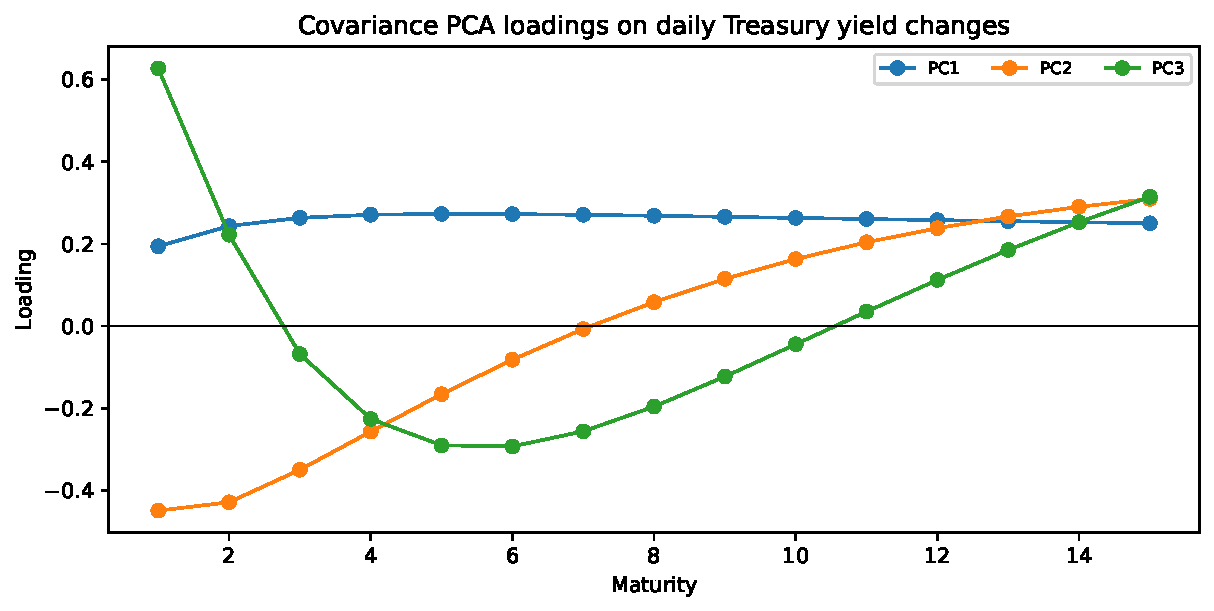
\includegraphics[width=0.92\textwidth]{figures/treasury_pca_loadings.pdf}
\caption{Covariance PCA loadings and explained variance. The first three components recover the
standard level, slope, and curvature shape.}
\label{fig:pca_loadings}
\end{figure}

The exact 2s5s10s butterfly solves for weights $w=(w_2,w_5,w_{10})$ such that
\begin{equation}
    w^\top L_1=0, \qquad w^\top L_2=0, \qquad w_5=-1.
\end{equation}
The spread is
\begin{equation}
    s_t = w_2 y_{2,t} + w_5 y_{5,t} + w_{10}y_{10,t}.
\end{equation}
The exact weights and regularized weights are reported together because their difference is the
central implementation lesson.

\begin{table}[H]
\centering
\scriptsize
\resizebox{0.68\textwidth}{!}{\input{generated/butterfly_weights.tex}}
\caption{Exact PC-neutral weights versus regularized weights. The belly is normalized to -1.}
\label{tab:weights}
\end{table}

\begin{table}[H]
\centering
\scriptsize
\resizebox{0.72\textwidth}{!}{\input{generated/butterfly_exposures.tex}}
\caption{PC exposures of exact and regularized butterfly weights. Regularization accepts small
level/slope exposure in exchange for lower gross and more stable weights.}
\label{tab:exposures}
\end{table}

\begin{figure}[H]
\centering
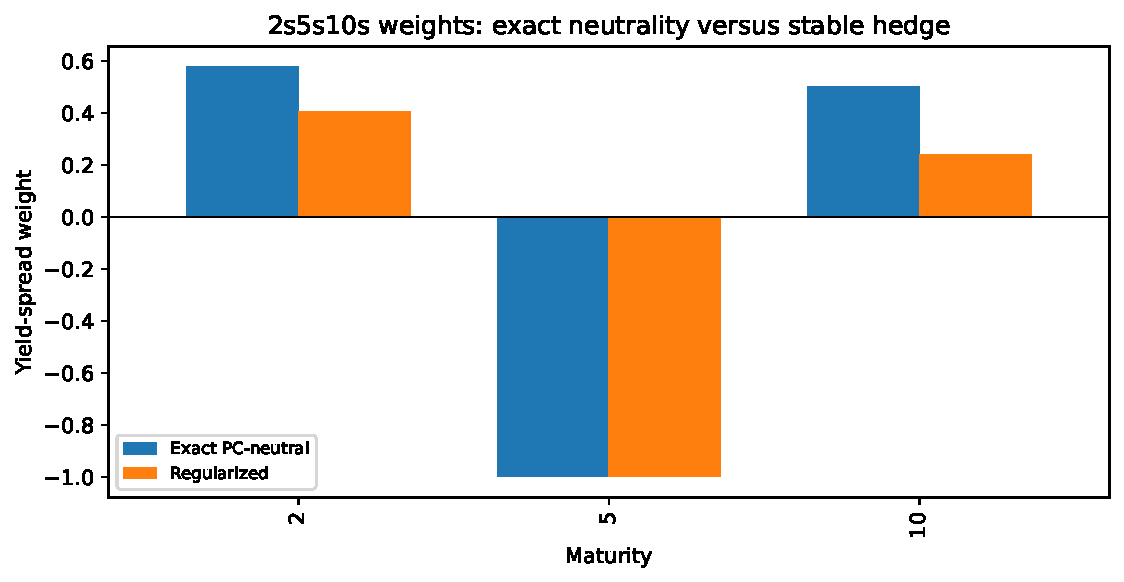
\includegraphics[width=0.78\textwidth]{figures/treasury_weight_comparison.pdf}
\caption{Exact PC-neutral weights versus regularized weights.}
\label{fig:weight_comparison}
\end{figure}

\section{Stationarity, Hedge Stability, and Carry}\label{sec:stationarity}

The exact construction works mechanically: it neutralizes PC1 and PC2 and keeps curvature exposure.
That is not enough. The exact static spread has an ADF p-value of 0.1669 and an
estimated half-life of about 1,222 trading days. The regularized spread is even more persistent by
this diagnostic. A residual this slow should not be treated as a high-confidence mean-reversion
trade.

\begin{table}[H]
\centering
\scriptsize
\resizebox{\textwidth}{!}{\input{generated/stationarity_summary.tex}}
\caption{Stationarity diagnostics for exact and regularized fixed-maturity spreads.}
\label{tab:stationarity}
\end{table}

Walk-forward estimation exposes the second problem. Exact rolling PCA weights can become very
large because local loadings shift. The full-sample exact trade is elegant; the rolling exact trade is
fragile. Regularization changes the decision from ``zero exposure at any cost'' to ``small residual
exposure with bounded gross.'' The monthly regularized hedge averages 0.3993, -1.0000, and
0.2363 on the 2Y, 5Y, and 10Y legs, with average gross exposure of 1.6356 and a maximum of
1.8607.

\begin{table}[H]
\centering
\scriptsize
\resizebox{\textwidth}{!}{\input{generated/rolling_regularized_summary.tex}}
\caption{Walk-forward regularized weight and residual exposure summary.}
\label{tab:rolling_regularized}
\end{table}

\begin{figure}[H]
\centering
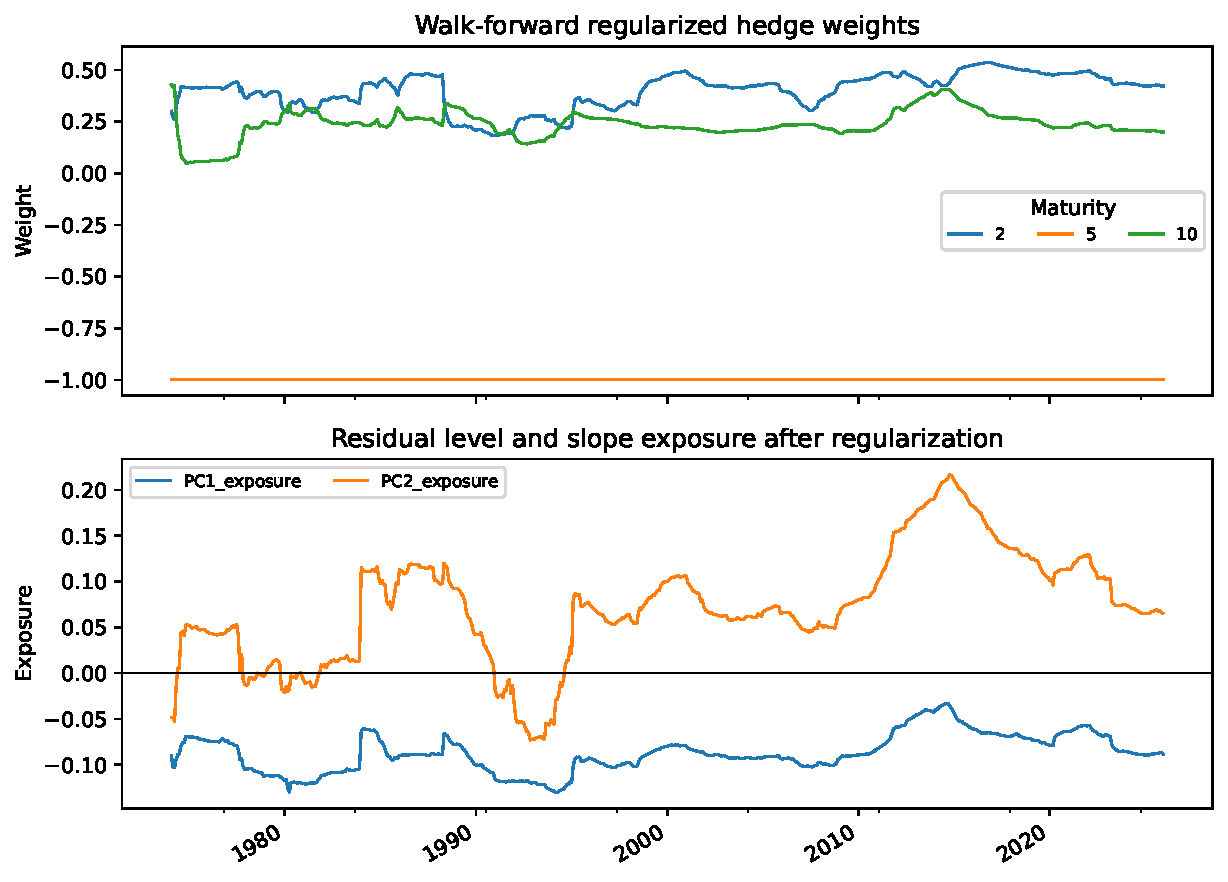
\includegraphics[width=0.94\textwidth]{figures/treasury_rolling_regularized_weights.pdf}
\caption{Walk-forward regularized weights, residual PC exposures, and gross notional.}
\label{fig:rolling_regularized}
\end{figure}

Carry enters because a curve trade can look statistically cheap while the curve's own rolldown
pushes against it. The research proxy uses unchanged-curve rolldown of the weighted yield spread.
It is not full bond carry, but it is enough to prevent the strategy from blindly fading a persistent
spread when the curve shape pays the opposite direction.

\begin{figure}[H]
\centering
\includegraphics[width=0.94\textwidth]{figures/treasury_signal_diagnostics.pdf}
\caption{Regularized curvature spread, lagged robust z-score, and unchanged-curve rolldown proxy.}
\label{fig:signal_diagnostics}
\end{figure}

\section{Investability Screen}\label{sec:investability}

The strategy layer tests two hypotheses. The first is residual mean reversion: fade rich or cheap
curvature after robust z-score, carry gating, volatility targeting, maximum holding periods, and
transaction costs. The second is carry-aligned curvature momentum: if the spread has been moving
and rolldown points the same way, follow the move rather than fight it.

\begin{table}[H]
\centering
\scriptsize
\resizebox{\textwidth}{!}{\input{generated/strategy_stats.tex}}
\caption{Strategy diagnostics. P\&L is a fixed-maturity research proxy in yield-spread bp.}
\label{tab:strategy_stats}
\end{table}

The table changes the story. Exact static mean reversion earns 303.35 bp with a 0.20 Sharpe, but
that result uses full-sample weights. Exact rolling mean reversion earns 988.63 bp with a near-zero
0.02 Sharpe and a -3,851.74 bp drawdown, so total P\&L is the wrong headline. The stricter
regularized mean-reversion variants lose money after costs. The carry-aligned momentum branch is
the least-rejected branch, not a strong strategy result. It earns 307.47 bp with a 0.18 Sharpe and
-125.14 bp max drawdown.

\begin{figure}[H]
\centering
\includegraphics[width=0.94\textwidth]{figures/treasury_strategy_pnl_drawdown.pdf}
\caption{Cumulative net P\&L and drawdown for regularized strategy hypotheses.}
\label{fig:strategy_pnl}
\end{figure}

These are not live-trading statistics. They are fixed-maturity, yield-space research diagnostics.
Their purpose is to decide which hypothesis deserves instrument-level work. On that standard,
mean reversion is rejected and carry-aligned momentum remains alive but modest.

\section{Robustness and Anti-Overfit Controls}\label{sec:robustness}

The main overfit risk is strategy selection. We therefore evaluate pre-declared
mean-reversion configurations and momentum horizons with chronological combinatorial purged
cross-validation. The purge length is 42 trading days, matching the maximum holding period, with
an additional five-day embargo around test windows. The folds are interpreted as Treasury-curve
regime blocks, not IID samples.

\begin{table}[H]
\centering
\scriptsize
\resizebox{\textwidth}{!}{\input{generated/strategy_cpcv_summary.tex}}
\caption{CPCV strategy diagnostics across pre-declared strategy families.}
\label{tab:cpcv}
\end{table}

The CPCV table reinforces the economic conclusion. Carry-aligned momentum ranks above the
mean-reversion family. The 21-day momentum variant has mean fold P\&L of 81.34 bp and positive
P\&L in 75\% of folds; the 63-day variant has mean fold P\&L of 76.87 bp and positive P\&L in
85.71\% of folds. The best mean-reversion families remain negative.

\begin{table}[H]
\centering
\scriptsize
\resizebox{\textwidth}{!}{\input{generated/null_simulation_summary.tex}}
\caption{Null simulations for the carry-aligned momentum branch. The full-curve null uses empirical
heavy-tailed innovations and EGARCH-style volatility clustering.}
\label{tab:nulls}
\end{table}

\begin{table}[H]
\centering
\scriptsize
\resizebox{0.74\textwidth}{!}{\input{generated/tail_diagnostics.tex}}
\caption{Student-t tail diagnostics for daily yield changes.}
\label{tab:tails}
\end{table}

\begin{figure}[H]
\centering
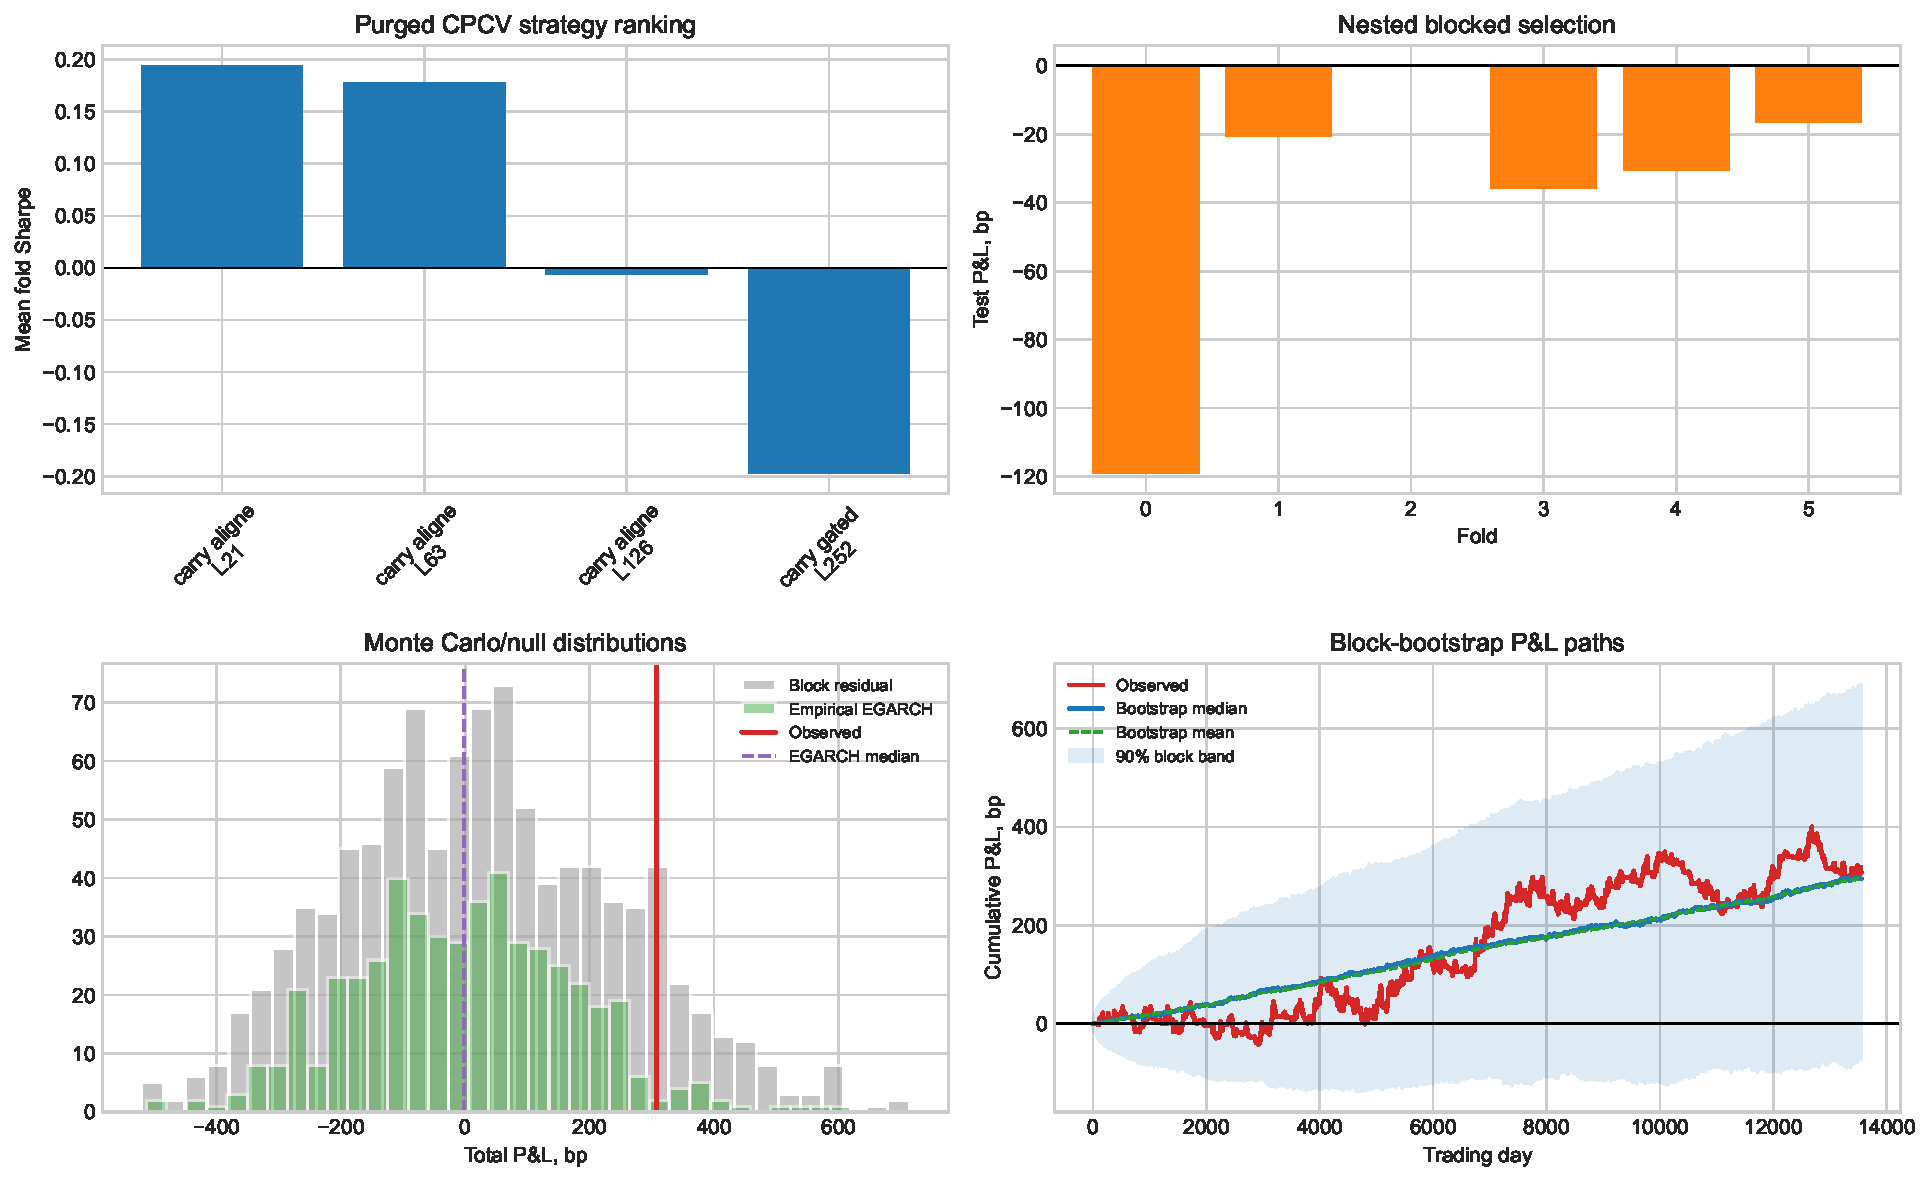
\includegraphics[width=0.96\textwidth]{figures/treasury_robustness_summary.pdf}
\caption{Robustness dashboard: CPCV strategy ranking, nested selected mean-reversion tests,
empirical EGARCH full-curve nulls, and block-bootstrap cumulative P\&L paths.}
\label{fig:robustness}
\end{figure}

The validation layer is intentionally conservative. Under the factor-residual block bootstrap, the
observed carry-momentum P\&L has one-sided p-values of 0.08 on total P\&L and 0.08 on Sharpe.
Under the empirical EGARCH full-curve null, the p-values are 0.09 and 0.10 in the regenerated
public artifacts. This is encouraging enough to keep the branch alive, but not strong enough to
call it validated production alpha.

\section{Bond Implementation and Production Gap}\label{sec:implementation}

Fixed-maturity yields are clean research objects. Trades are done in bonds, futures, swaps, or
packages. The repo therefore maps monthly rebalances to nearby Treasury bonds around the 2Y,
5Y, and 10Y targets and compares selected-bond yield changes against GSW fixed-maturity changes.
This is where many curve-RV projects become unrealistic.

\begin{table}[H]
\centering
\scriptsize
\resizebox{\textwidth}{!}{\input{generated/bond_mapping_summary.tex}}
\caption{Nearest-bond mapping quality by target tenor.}
\label{tab:bond_mapping}
\end{table}

\begin{table}[H]
\centering
\scriptsize
\resizebox{\textwidth}{!}{\input{generated/bond_tracking_error_summary.tex}}
\caption{Selected-bond yield-change tracking error versus fixed-maturity targets.}
\label{tab:bond_tracking}
\end{table}

\begin{figure}[H]
\centering
\includegraphics[width=0.92\textwidth]{figures/treasury_bond_mapping.pdf}
\caption{Actual-bond implementation diagnostics: maturity gap and fixed-maturity tracking error.}
\label{fig:bond_mapping}
\end{figure}

The tracking error is not catastrophic, but it is not zero. The 2Y, 5Y, and 10Y selected-bond RMSEs
are about 8.41, 8.00, and 7.35 bp. A production version would need DV01 sizing, coupon and
benchmark selection, bid/ask, repo and financing, accrued interest, roll mechanics, futures CTD
logic if implemented through futures, and portfolio-level risk controls. Those are not cosmetic
details. They decide whether the fixed-maturity signal survives the instrument layer.

\section{Conclusion}\label{sec:conclusion}

Through this sequence, we can conclude that a PCA-neutral Treasury butterfly is a useful
construction but not a strategy by itself. The factor model works: Treasury yield changes are
dominated by level, slope, and curvature, and exact 2s5s10s weights can neutralize level and slope.
The trade thesis is weaker. The residual is not strongly stationary, exact rolling hedge ratios are
unstable, and stricter mean-reversion variants lose money after costs.

The final conclusion is bounded. Regularized hedge construction produces stable weights, and
carry-aligned curvature momentum is more plausible than naive z-score fading. The anti-overfit layer
keeps that branch alive but does not promote it to live alpha. A production version would need DV01
sizing, benchmark or CTD selection, bid/ask, repo and financing, roll mechanics, and portfolio-level
risk controls. The result is useful because it shows the full research path: build the factor trade,
test the attractive story, reject what fails, and state clearly what still has to be true before
capital can be put behind it.

\begin{thebibliography}{9}
\bibitem{littermanscheinkman1991} Litterman, R. and Scheinkman, J. (1991). Common factors affecting bond returns. \textit{Journal of Fixed Income}, 1(1):54--61.
\bibitem{cochranepiazzesi2005} Cochrane, J. H. and Piazzesi, M. (2005). Bond risk premia. \textit{American Economic Review}, 95(1):138--160.
\bibitem{duartelongstaffyu2007} Duarte, J., Longstaff, F. A., and Yu, F. (2007). Risk and return in fixed-income arbitrage: Nickels in front of a steamroller? \textit{Review of Financial Studies}, 20(3):769--811.
\bibitem{neweywest1987} Newey, W. K. and West, K. D. (1987). A simple, positive semi-definite, heteroskedasticity and autocorrelation consistent covariance matrix. \textit{Econometrica}, 55(3):703--708.
\bibitem{lopezdeprado2018} Lopez de Prado, M. (2018). \textit{Advances in Financial Machine Learning}. Wiley.
\bibitem{engle1982} Engle, R. F. (1982). Autoregressive conditional heteroscedasticity with estimates of the variance of United Kingdom inflation. \textit{Econometrica}, 50(4):987--1007.
\bibitem{gurkaynak2007} Gurkaynak, R. S., Sack, B., and Wright, J. H. (2007). The U.S. Treasury yield curve: 1961 to the present. \textit{Journal of Monetary Economics}, 54(8):2291--2304.
\bibitem{fleming2003} Fleming, M. J. (2003). Measuring Treasury market liquidity. \textit{Economic Policy Review}, 9(3):83--108.
\end{thebibliography}

\end{document}
